\chapter{Manual Screen}
\section{Overview} \paragraph*{The}\textbf{\textit{Manual Screen}} is the screen the Operator navigates to in order to perform manual operations with the saw. The \textbf{\textit{Manual Screen}} cannot hold controls and indicators for all controlled devices on one screen. Therefore, the manual controls are divided over several screens that are accessable from the \textbf{\textit{Manual Screen}}. This is described in detail below.
\begin{figure}
	\centering
	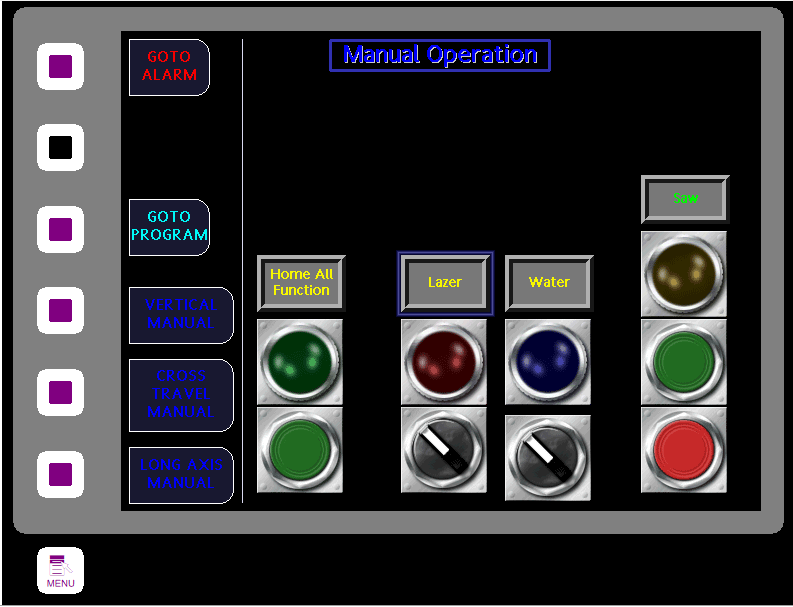
\includegraphics[width=0.5
	\linewidth]{screen-captures/manual/manual}
	\caption{Manual Screen}
	\label{fig:manual-screen}
\end{figure}
\pagebreak
\begin{figure}
	\centering
	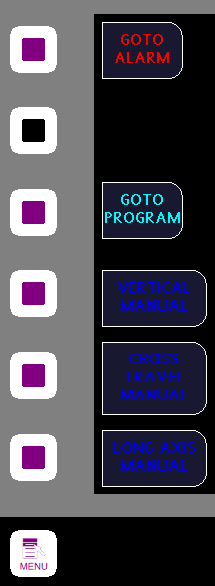
\includegraphics[width=.3\linewidth]{screen-captures/manual/manual-nav}
	\caption{Manual Screen Navigation}
	\label{fig:manual-nav}
\end{figure}
\section{Manual Screen Details}
\paragraph*{The}\textbf{\textit{Manual Screen}} details are divided into the following categories.
\begin{list}{$\diamond$}{}
	\item \textbf{Screen Navigation}
	\item \textbf{Home All}
	\item \textbf{Lazer}
	\item \textbf{Water}
	\item \textbf{Saw}
\end{list}
\subsection{Screen Navigation}\paragraph*{Is}performed by using the programmable Function Keys (FKeys) located down the left hand side of the OI Terminal (refer to Figure 3.2). The Operator may navigate to the \textbf{\textit{Alarm Screen}} and the \textbf{\textit{Program Screen}} and of course the \textbf{\textit{Main Screen}} using the \textit{Menu} FKey. As well, there are navigation keys programmed for going to the manual control screens for Long, Cross, and Vertical axii.
\begin{list}{$\diamond$-}{}
	\item \textbf{GOTO ALARM} Navigate to Manual Screen.
	\item \textbf{GOTO PROGRAM} Navigate to Cut Program Screen.
	\item \textbf{VERTICAL MANUAL} Navigate to Vertical Axis Manual Control Screen.
	\item \textbf{CROSS TRAVEL MANUAL} Navigate to Cross Travel Manual Control Screen.
	\item \textbf{LONG AXIS MANUAL} Navigate to the Long Axis Manual Control Screen.
\end{list}
\paragraph{\textbf{\LARGE \textcolor{blue}{i}}}
The Menu Key located on the terminal at the lower left below the FKey's, will return the Operator to the Main Screen, from all other screens.\\
\begin{minipage}{4cm}
	\begin{picture}(20,70)
	
\includegraphics[width=.5\linewidth]{screen-captures/menu}
	\end{picture}
\end{minipage}\begin{minipage}[]{11cm}
	\paragraph{\textbf{\LARGE \textcolor{blue}{i}}} The Menu Key is pictured as it looks on the Terminal.
\end{minipage}
\pagebreak
\begin{figure}
	\centering
	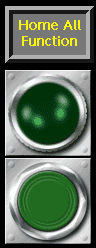
\includegraphics[width=.2\linewidth]{screen-captures/manual/manual-home-all}
	\caption{Manual Home All Function}
	\label{fig:manual-home-all}
\end{figure}
\subsection{Home All Function}\paragraph*{}Referring to Figure 3.3. The \textbf{\textit{Home All Function}} is actually a state of the saw, and this has special ramifications over the control of the saw. When a Home All command is initiated, providing there are no critical Fault conditions preventing the state from changing, the saw control system changes to that state. This precludes \textit{Hand/Auto} modes entirely, and prevents \textit{\textbf{Cut Program}} entry until the \textit{\textbf{Home All Function}} has completed. When initiated, the function will command the following ...
\begin{list}{$\diamond$}{}
	\item \textbf{Saw Off} Turn Off Saw Motor.
	\item \textbf{Disable Drives} Disable Vertical, Cross, and Long Drives.
	\item \textbf{Water Off} Turn Off Water Solenoid.
	\item \textbf{Enable Vertical} Enable Vertical Axis.
	\item \textbf{Home Vertical} Home Vertical Axis.
	\item \textbf{Enable Cross Travel} Enable Cross Travel Axis.
	\item \textbf{Home Cross Travel} Home Cross Travel Axis.
	\item \textbf{Enable Long} Enable Long Axis.
	\item \textbf{Home Long Axis} Home Long Axis.
	\item \textbf{Home Complete} Home Complete Indication.
\end{list}
Once Homing has begun, it continues through a predetermined sequence, until all motion has stopped and completed. Then Home Complete is acquired, and indicated to the control program. At this time the Saw transitions from the Homing State into the At Rest state. The mode will be whatever mode was active when entering the Homing State, and since Home can only be initiated from \textit{Hand} mode, this will always be \textit{Hand} mode. The \textbf{\textit{Home All Function}} is made up of the \textbf{\textit{Home PB}} and the \textbf{\textit{Home All Indicator}}. When not homed completely (if homed by individual commands), or if \textbf{\textit{Home All Function}} has not been completed, the \textbf{\textit{Home All Indicator}} will be off. During the \textbf{\textit{Home All Function}} executing, the \textbf{\textit{Home All Indicator}} will be blinking. When all axii are at \textbf{Home} the \textbf{\textit{Home All Indicator}} will be on solid.
\paragraph{\textbf{\LARGE \textcolor{blue}{i}}}The \textbf{\textit{Home All Function}} is a semi-automatic operation initiated by the Operator. Once initiated, it progresses through a predetermined sequence of operations to achieve the reference positions for all axii. This is irrespective of mode, and will only be stopped by completing the function, or a critical fault condition (including emergency stop), or a \textbf{\textit{Machine Full Stop}} pushbutton press.
\paragraph{\textbf{{\LARGE \textcolor{red}{!}}}} While pressing the \textbf{Emergency Stop PB} will trigger a Faulted condition that would result in the \textbf{\textit{Home All Function}} stopping, the \textbf{Safety Gate} Interlock circuit does not. Due to the nature of setting up and maintaining the Saw, it is necessary to have motion capabilities with the \textbf{Safety Gate} Interlock open. This includes the \textbf{\textit{Home All Function}} which constitutes the first steps of setting up the saw. As a consequence, it is important for the Operator to be aware that the \textbf{\textit{Home All Function}} may cause motion to occur automatically while the \textbf{Safety Gate} Interlock is open. The Operator \textbf{must} ensure the path of the Saw is unobstructed, and that no personnel are in the area of saw travel before initiating a \textbf{\textit{Home All Function}}.
\pagebreak
\begin{figure}
	\centering
	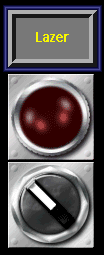
\includegraphics[width=.2\linewidth]{screen-captures/manual/manual-lazer}
	\caption{Manual Lazer Control}
	\label{fig:manual-lazer}
\end{figure}
\subsection{Lazer}\paragraph*{The}\textbf{\textit{Lazer}} Control is a selector switch that the Operator can use to turn on/off the Lazer. This is used during set up and entry of the cut program. Normally, the Lazer is off during operations. The red \textbf{Lazer Indicator} will turn on if the \textbf{\textit{Lazer}} is on, otherwise it is off.
\paragraph{\textbf{{\LARGE \textcolor{red}{!}}}} The Lazer optics used on this Lazer are industrial rated optics. The Operator, and personell working in the vicinity, should \textbf{never} look directly at the lazer light without appropriate eye protection as this \textbf{will} result in damage to the eye. If using the Lazer for cut location, keep your back facing the Lazer light source, and turn it off when you're not needing to use it.
\paragraph{\textbf{\LARGE \textcolor{blue}{i}}} The \textbf{\textit{Lazer}} is a handy tool during cut program set up. If turned on in \textit{Hand} mode, it will remain on until turned off by he Operator, or until the mode is switched to \textit{Auto}. As the \textbf{\textit{Lazer}} is not needed during cut program running, it does not run in \textit{Auto} mode.
\pagebreak
\begin{figure}
	\centering
	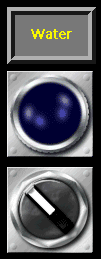
\includegraphics[width=.2\linewidth]{screen-captures/manual/manual-water}
	\caption{Manual Water Control}
	\label{fig:manual-water}
\end{figure}
\subsection{Water}\paragraph*{The}manual \textbf{\textit{Water}} control is a selector switch and indicator light, please refer to Figure 3.5. When the selector switch is in the On position (right) the \textbf{\textit{Water}} solenoid is turned on and once water flow is verified the \textbf{Indicator} will turn on. During \textit{Hand} mode operation, it is useful to be able to turn the water On/Off to verify solenoid and flow sensor operation. During \textit{Auto} mode operations, the water solenoid and the state of the flow switch monitoring, is controlled by the PLC.
\paragraph{\textbf{\LARGE \textcolor{blue}{i}}}Turning the water on and off in the Manual Screen is an easy way to test solenoid and flow switch operation prior to starting an Auto Cycle.
\paragraph{\textbf{{\LARGE \textcolor{red}{!}}}}If the \textbf{Flow Switch} does not indicate water flow while the selector switch is on, verify there is actual water flow, if not verify solenoid operation. If solenoid operation is verified, and water is not flowing establish proper flow then continue. Once flow is verified, and switch is still not operating, check switch for correct operation and replace if necessary. Without water flow demand and indication, \textbf{\textit{Cut Program}} automatic execution is inhibited.
\pagebreak
\begin{figure}
	\centering
	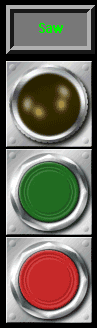
\includegraphics[width=.2\linewidth]{screen-captures/manual/manual-saw}
	\caption{Manual Saw Control}
	\label{fig:manual-saw}
\end{figure}
\subsection{Saw}\paragraph*{The}manual \textbf{\textit{Saw}} control is made up of a \textbf{Start} pushbutton, a \textbf{Stop} pushbutton, and an amber \textbf{Indicator} pilot light. In order to be able to \textbf{Start} the Saw motor, the \textbf{Safety Gate} interlocks \textbf{must} be closed, and the safety circuit satisfied. Pressing \textbf{Start} will begin start up of the saw motor. Since the blade is a rather large inertial load, start up is gradual and should be allowed for. Once the saw blade motor is running, the amber \textbf{Indicator} pilot light will turn on. The exact point at which the \textbf{Indicator} comes on is determined by the saw motor Soft Start \textbf{Run} contact, and may not repesent full motor speed. To stop the saw blade motor, press the \textbf{Stop} pushbutton. The \textbf{Indicator} pilot light will turn off.
\paragraph{\textbf{{\LARGE \textcolor{red}{!}}}}The saw blade motor does not have a brake on it, and since the saw blade is a large inertial load, the entire rotating mass will take some noticeable time to come to a complete stop. Personell \textbf{must} wait for the saw blade to come to a complete standstill before entering the saw work area.
\paragraph{\textbf{\LARGE \textcolor{blue}{i}}}The saw motor operation in \textit{Auto} mode is done by the program control, not by direct Operator input. When the \textit{Auto} cycle is started, the motor is turned on and after a time delay and run confirmation, the water is turned on. Once flow is established the Automatic Run State is entered.